\documentclass[tikz,border=10pt]{standalone}
\usepackage{tikz}
\usetikzlibrary{arrows.meta,positioning}

\tikzset{
  card/.style={draw=blue!70!black, line width=1.2pt, rounded corners=3pt, minimum width=6.2cm, minimum height=1.0cm, align=center, fill=none},
  warn/.style={draw=orange!80!black, line width=1.2pt, rounded corners=3pt, minimum width=6.2cm, minimum height=1.0cm, align=center, fill=none},
  flow/.style={-{Stealth[length=3mm]}, line width=1.2pt, draw=black!70}
}

\begin{document}
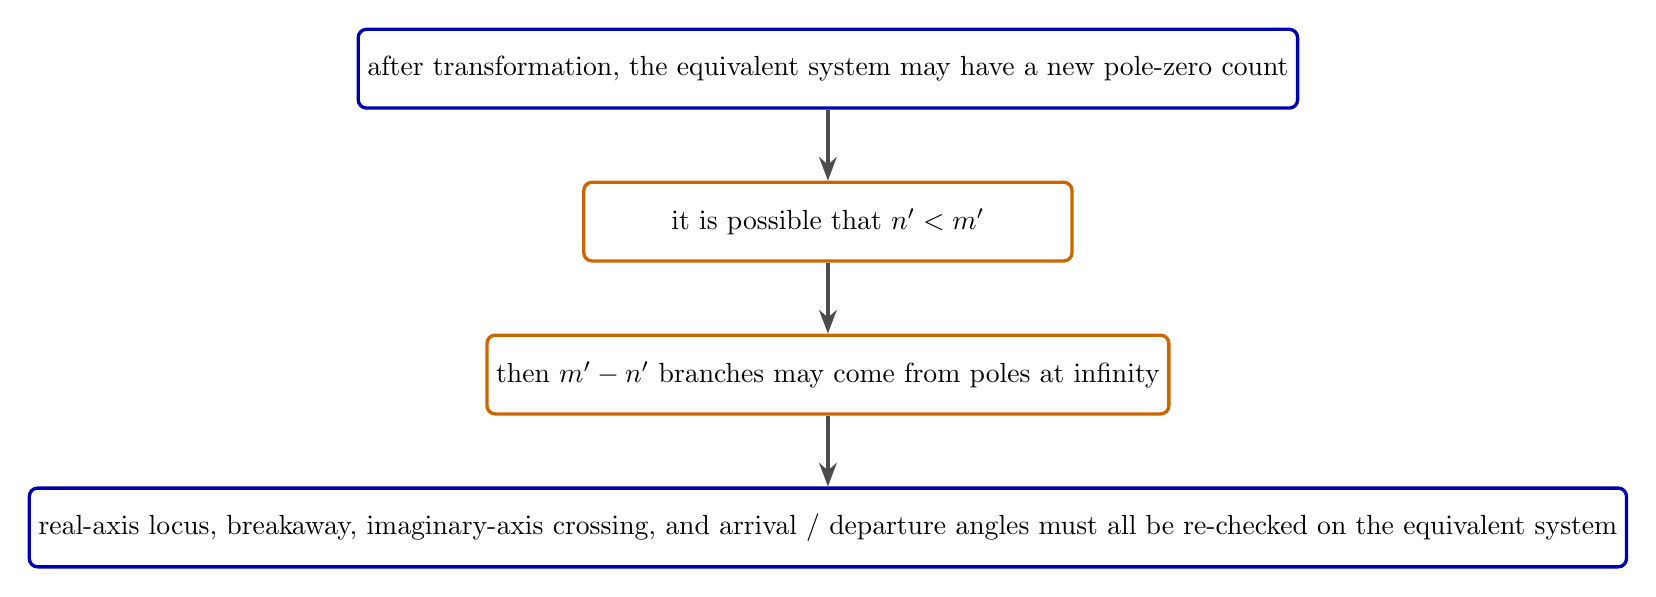
\begin{tikzpicture}[node distance=0.9cm]
  \node[card] (a) {after transformation, the equivalent system may have a new pole-zero count};
  \node[warn, below=of a] (b) {it is possible that $n' < m'$};
  \node[warn, below=of b] (c) {then $m'-n'$ branches may come from poles at infinity};
  \node[card, below=of c] (d) {real-axis locus, breakaway, imaginary-axis crossing, and arrival / departure angles must all be re-checked on the equivalent system};

  \draw[flow] (a) -- (b);
  \draw[flow] (b) -- (c);
  \draw[flow] (c) -- (d);
\end{tikzpicture}
\end{document}
